\newpage
\section{Utilisation des styles}
\subsection{Définition de \tkzcname{tkzTabSetup}}

Le plus simple est d'utiliser la macro  \tkzcname{tkzTabSetup}. Celle-ci permet de modifier les styles principaux.

\begin{NewMacroBox}{tkzTabSetup}{\oarg{local options}}

\begin{tabular}{llc}
\toprule
\texttt{arguments}   & \texttt{défaut}    & \texttt{définition}                 \\
\midrule
\IargName{tkzTabSetup}{doubledistance} & |1pt| & écart double barre         \\
\IargName{tkzTabSetup}{doublecolor}  & |white|  & couleur centrale dans la double barre         \\
\IargName{tkzTabSetup}{lw}  & |0.4pt| & épaisseur d'un trait                \\
\IargName{tkzTabSetup}{color}  & |black| & couleur d'un trait               \\
\midrule
\IargName{tkzTabSetup}{tstyle}  & |dotted|  & style des traits verticaux        \\
\IargName{tkzTabSetup}{tcolor  } & |black| & couleur des  traits verticaux       \\
\IargName{tkzTabSetup}{tanarrowstyle}&|latex'|&style d'une flèche pour une tangente  \\
\IargName{tkzTabSetup}{tanstyle}& |->| & style  d'une tangente              \\
\IargName{tkzTabSetup}{tancolor}& |black| & couleur d'une tangente          \\
\IargName{tkzTabSetup}{tanwidth}& |0.4pt|& épaisseur d'une tangente         \\
\IargName{tkzTabSetup}{fromarrowstyle}&|latex'|&style d'une flèche antécédent -> image   \\
\IargName{tkzTabSetup}{fromstyle }& |->|  & style antécédent -> image              \\
\IargName{tkzTabSetup}{fromcolor }& |black|  & couleur antécédent -> image         \\
\IargName{tkzTabSetup}{fromwidth }& |0.4pt|  & épaisseur  antécédent -> image      \\
\IargName{tkzTabSetup}{hcolor   } & |gray|  & couleur d'une zone interdite        \\
\IargName{tkzTabSetup}{hopacity } & |0.4|  & transparence de la couleur d'une zone interdite         \\
\IargName{tkzTabSetup}{crosslines}& |false|  & booléen true hachure la zone interdite  \\
\IargName{tkzTabSetup}{arrowcolor}& |black|  & couleur d'une flèche de variation     \\
\IargName{tkzTabSetup}{arrowstyle}& |latex'| & style d'une flèche de variation     \\
\IargName{tkzTabSetup}{arrowlinewidth}&|0.4pt|&épaisseur d'une flèche de variation  \\
\bottomrule
\end{tabular}

\medskip
\noindent\emph{Cette macro s'utilise dès le début. Les épaisseurs sont en générale donnée en \tkzname{pt}, la valeur par défaut est la plus fréquente. }

\end{NewMacroBox}

\subsubsection{Utilisation de \tkzname{doubledistance} et  \tkzname{hcolor}}

\begin{center}
\begin{tikzpicture}
   \tkzTabColors[backgroundcolor=fondpaille,%
             color=Maroon]
  \tkzTabSetup[doubledistance = 2pt]
  \tkzTabInit[lgt=2,espcl=1]
  {$x$         /1, $x^2-3x+2$   /1, $\ln (x^2-1)$  /1,  $E(x)$       /1}%
  {$-\infty$ ,$-\sqrt{2}$, $-1$ , $1$ ,$\sqrt{2}$ , $2$ , $+\infty$}%
  \tkzTabLine{ , + , t , + , t , + , z , - , t , - , z , + , }
  \tkzTabLine{ , + , z , - , d , h , d , - , z , + , t , + , }
  \tkzTabLine{ , + , z , - , d , h , d , +  ,z , - , z , + , }
\end{tikzpicture}
\end{center}


\begin{tkzexample}[code only,small]
\begin{tikzpicture}
 \tkzTabColors[backgroundcolor=fondpaille,%
           color=Maroon]
\tkzTabSetup[doubledistance = 2pt]
\tkzTabInit[lgt=2,espcl=1]
{$x$         /1, $x^2-3x+2$   /1, $\ln (x^2-1)$  /1,  $E(x)$       /1}%
{$-\infty$ ,$-\sqrt{2}$, $-1$ , $1$ ,$\sqrt{2}$ , $2$ , $+\infty$}%
\tkzTabLine{ , + , t , + , t , + , z , - , t , - , z , + , }
\tkzTabLine{ , + , z , - , d , h , d , - , z , + , t , + , }
\tkzTabLine{ , + , z , - , d , h , d , +  ,z , - , z , + , }
\end{tikzpicture}
\end{tkzexample}

\subsubsection{Utilisation de \tkzname{fromcolor} et  \tkzname{tancolor}}

\begin{center}
	\begin{tikzpicture}
	 \tkzTabSetup[fromcolor        = red, tancolor         = blue,,backgroundcolor=fondpaille,%
	             color=Maroon]
	 \tkzTabInit[espcl=4]
	    { $x$          /1,  $f''(x)$     /1,  $f'$      /3, $f$       /4}%
	    { $0$      , $1$ ,     $\alpha$,$+\infty$ }%
	 \tkzTabLine {d    , + ,   z  , -  ,      , -  }%
	 \tkzTabVar
	   {- / $1$       /,  + /           /,  R /           /, - / $-\infty$ /}

	 \tkzTabVal[draw]{2}{4}{0.5}{}{0}
	 \tkzTabIma[draw]{2}{4}{3}{$0$}
	 \tkzTabTan[pos]{1}{2}{2}{$2$}
	 \tkzTabVar
	    {- / $-\infty$ ,  R /  , + / $1$ , - / $0$       }
	  \tkzTabIma[draw]{1}{3}{2}{$0$}
	\end{tikzpicture}
\end{center}


\begin{tkzexample}[code only,small]
\begin{tikzpicture}
 \tkzTabSetup[fromcolor        = red, tancolor         = blue,,backgroundcolor=fondpaille,%
             color=Maroon]
 \tkzTabInit[espcl=4]
    { $x$          /1,  $f''(x)$     /1,  $f'$      /3, $f$       /4}%
    { $0$      , $1$ ,     $\alpha$,$+\infty$ }%
 \tkzTabLine {d    , + ,   z  , -  ,      , -  }%
 \tkzTabVar
   {- / $1$       /,  + /           /,  R /           /, - / $-\infty$ /}

 \tkzTabVal[draw]{2}{4}{0.5}{}{0}
 \tkzTabIma[draw]{2}{4}{3}{$0$}
 \tkzTabTan[pos]{1}{2}{2}{$2$}
 \tkzTabVar
    {- / $-\infty$ ,  R /  , + / $1$ , - / $0$       }
  \tkzTabIma[draw]{1}{3}{2}{$0$}
\end{tikzpicture}
\end{tkzexample}

\subsection{Utilisation de \tkzcname{tikzset} pour modifier les styles}

Voici la liste des styles qui sont utilisés et leurs définitions.

\begin{tabular}{ll}
\toprule
\tkzname{node style} & style des nodes utilisé pour les valeurs placées dans le tableau  \\
\tkzname{low left} &  valeur située en bas et à gauche d'un trait vertical  \\
\tkzname{low right} & valeur située en bas et à droite d'un trait vertical\\
\tkzname{hight left} & valeur située en haut et à gauche d'un trait vertical\\
\tkzname{hight right}& valeur située en haut et à droite d'un trait vertical\\
\tkzname{low} & valeur située en bas d'un trait vertical \\
\tkzname{hight } & valeur située en haut d'un trait vertical \\
\tkzname{on double} & couleur du fond sous une double barre \\
\tkzname{tan style} & style pour une tangente\\
\tkzname{arrow style} & style pour les flèches des variations\\
\tkzname{from style} & style pour la ligne allant d'un antécédent à une image\\
\tkzname{h style} & style pour une zone interdite\\
\tkzname{double style} & style pour une double barre\\
\tkzname{t style} & style pour un trait vertical\\
\bottomrule
\end{tabular}


Les valeurs par défaut utilisées sont les suivantes :
\begin{tkzexample}[code only, small]
\def\tkzTabDefaultWritingColor{black}
\def\tkzTabDefaultBackgroundColor{white}
\def\tkzTabDefaultLineWidth{0.4pt}
\def\tkzTabDefaultArrowStyle{latex'}
\def\tkzTabDefaultSep{2pt}
\end{tkzexample}

les principaux styles par défaut sont :

\begin{tkzexample}[code only, small]
\tikzset{node style/.style  = {inner sep   =  \tkzTabDefaultSep,
                               outer sep   =  \tkzTabDefaultSep,
                               fill        =  \tkzTabDefaultBackgroundColor}}
\tikzset{tan style/.style   = {>           =  \tkzTabDefaultArrowStyle,
                               ->,
                               color       =  \tkzTabDefaultBackgroundColor}}
\tikzset{arrow style/.style = {\tkzTabDefaultWritingColor,
                               ->,
                               >            = \tkzTabDefaultArrowStyle,
                               shorten >    = \tkzTabDefaultSep,
                               shorten <    = \tkzTabDefaultSep}}
\tikzset{from style/.style   = {shorten >   = \tkzTabDefaultSep,
                                shorten <   = \tkzTabDefaultSep,
                                line width  = \tkzTabDefaultLineWidth,
                                >           = \tkzTabDefaultArrowStyle,
                                ->,
                                draw        = \tkzTabDefaultWritingColor,
                                dotted}}
\tikzset{t style/.style = {style  = dotted,
                           draw   = \tkzTabDefaultWritingColor}}
\tikzset{h style/.style = {pattern       = north west lines,
                           pattern color = \tkzTabDefaultWritingColor}}
\tikzset{on double/.style   = {fill      =  \tkzTabDefaultBackgroundColor}}
\tikzset{double style/.append style = {%
         draw            = \tkzTabDefaultWritingColor,
         double          =  \tkzTabDefaultBackgroundColor}}
\end{tkzexample}

Les couleurs de fond pour les différentes sont définies par les styles :
\begin{tkzexample}[code only, small]
\tikzset{fondC/.style={fill = \tkzTabDefaultBackgroundColor}}
\tikzset{fondL/.style={fill = \tkzTabDefaultBackgroundColor}}
\tikzset{fondT/.style={fill = \tkzTabDefaultBackgroundColor}}
\tikzset{fondV/.style={fill = \tkzTabDefaultBackgroundColor}}
\end{tkzexample}
Enfin les approches des valeurs par les flèches sont :
\begin{tkzexample}[code only, small]
\tikzset{low left/.style    = {above left  =  \tkzTabDefaultSep}}
\tikzset{low right/.style   = {above right =  \tkzTabDefaultSep}}
\tikzset{high right/.style  = {below right =  \tkzTabDefaultSep}}
\tikzset{high left/.style   = {below left  =  \tkzTabDefaultSep}}
\tikzset{low/.style         = {above       =  \tkzTabDefaultSep}}
\tikzset{high/.style        = {below       =  \tkzTabDefaultSep}}
\end{tkzexample}

\subsubsection{Utilisation de \tkzcname{tikzset} et \tkzname{h style}}


\begin{tkzexample}[latex=8cm,small]
\begin{tikzpicture}
  \tkzTabColors[backgroundcolor=fondpaille,%
                color=Maroon]
  \tkzTabSetup[doubledistance = 2pt]
  \tikzset{h style/.style = {fill=red!50}}
  \tkzTabInit[color,espcl=1.5]%
    {$x$ / 1,$g(x)$ / 1}%
    {$0$,$1$,$2$,$3$}%
  \tkzTabLine{z,+,d,h,d,-,t}
\end{tikzpicture}
\end{tkzexample}

\subsubsection{Utilisation de \tkzcname{tikzset} et \tkzname{h style}}

\begin{tkzexample}[latex=8cm,small]
\begin{tikzpicture}
\tikzset{h style/.append style = {%
         pattern=north east lines}}
\tkzTabInit[color,espcl=1.5]%
    {$x$ / 1,$g(x)$ / 1}%
    {$0$,$1$,$2$,$3$}%
\tkzTabLine{z,+,,h,d,-,t}
\end{tikzpicture}
\end{tkzexample}

\subsubsection{Utilisation de \tkzcname{tikzset} et \tkzname{arrow style}}

\begin{center}
	\begin{tkzexample}[vbox,small]
	  %\newcommand*{\E}{\ensuremath{\mathrm{e}}}
	\begin{tikzpicture}

	\tikzset{arrow style/.append style = {red,shorten >=6pt,shorten <=6pt}}
	\tkzTabInit[espcl=5]{$x$ /1, $\ln x +1$ /1.5, $x \ln x$ /2}%
	{$0$ ,$1/\E$ , $+\infty$}%
	\tkzTabLine{d,-,z,+,}
	\tkzTabVar%
	{ D+/ / $0$ ,%
	-/ \colorbox{black}{\textcolor{white}{$\dfrac{-1}{e}$}}/ ,%
	+/ $+\infty$ / }%
	\end{tikzpicture}
	\end{tkzexample}
\end{center}


\subsubsection{Utilisation de \tkzcname{tikzset} et \tkzcname{tkzTabSetup}}

 On remarquera la dernière utilisation de   \tkzcname{tkzTabSetup} qui remet les valeurs par défaut.

\begin{center}
	\begin{tkzexample}[vbox,small]
	% \newcommand*{\va}{\colorbox{red!50}    {$\scriptscriptstyle V_a$}}
	% \newcommand*{\vb}{\colorbox{blue!50}   {$\scriptscriptstyle V_b$}}
	% \newcommand*{\vc}{\colorbox{gray!50}   {$\scriptscriptstyle V_c$}}
	% \newcommand*{\vd}{\colorbox{magenta!50}{$\scriptscriptstyle V_d$}}
	% \newcommand*{\ve}{\colorbox{orange!50} {$\scriptscriptstyle V_e$}}

	\begin{tikzpicture}
	\tkzTabSetup[fromcolor      =  red,
	            fromstyle       = dashed,
	            fromwidth       = 1pt,
	            fromarrowstyle  = stealth',
	            arrowcolor      = green ]
	  \tkzTabInit[lgt=1.5,espcl=5]{ $x$/.7,$f''(x)$/.7,$f'$/3,$f$/3 }%
	             {  $a$    , $d$    ,$e$}
	  \tkzTabLine{  z,+    ,z,-     ,z  }
	  \tkzTabVar  {-/\va  ,+/\vd   , -/  \ve}
	  \tkzTabVal[draw,remember=vb]{1}{2}{0.333}{b}{$1$}
	  \tikzset{from style/.append style = {draw      =  blue}}
	  \tkzTabVal[draw,remember=vc]{1}{2}{0.666}{c}{$2$}
	  \tkzTabVar{-/$-\infty$  ,R/   , +/  $+\infty$}
	  \tkzTabSetup
	  \tkzTabVal[draw]{1}{3}{0.5}{}{$0$}
	  \draw[opacity=0.5,fill=red!40]  (vb) circle(2ex);
	  \draw[opacity=0.5,fill=blue!40] (vc) circle(2ex);
	\end{tikzpicture}
	\end{tkzexample}
\end{center}



\endinput



